\documentclass[11pt]{article}

% Use wide margins, but not quite so wide as fullpage.sty
\marginparwidth 0.5in 
\oddsidemargin 0.25in 
\evensidemargin 0.25in 
\marginparsep 0.25in
\topmargin 0.25in 
\textwidth 6in \textheight 8 in
% That's about enough definitions

\usepackage{graphics}
\usepackage{ulem}
\usepackage{hyperref}
\hypersetup{
  colorlinks,
  citecolor=Violet,
  linkcolor=Red,
  urlcolor=blue}


\begin{document}
\hfill\vbox{\hbox{Ibssa, Girum}
		\hbox{Cpe 453, Section 02}	
		\hbox{Assignment 4}	
		\hbox{\today}}\par

\bigskip
\centerline{\Large\bf Assignment 4: Minix Secret Driver}\par
\bigskip

This is the template I passed out in the lab (well, slightly 
modified).  It works reasonably well to have each step of the
lab be a {\textbackslash section} and each component below it
a {\textbackslash subsection}.  For the ``problem set'' labs
an {\tt enumerate} environment is probably more appropriate.


\setcounter{section}{1} % make the first section, section 2(see below)

\section{Overall Architecture of the Driver}
% An overall architecture of the driver: How is it expected to function?
Minix uses a non-monolithic, message-based, callback framework for its kernel. A mouthful, but this just means that Minix is structured to be a very modular, framework-y codebase. This is great for me, since all I really have to do is write callback functions for \texttt{open(), close()} and \texttt{transfer()} to finish the assignment. To me, this means that all my Secret has to do is define handlers for:

\begin{itemize}
\item Parse the incoming \texttt{message *} for its sender's credentials in the callback for  \texttt{open()}.
\item Persist who said owner is globally.
\item Bounce users who try and access my Secret if they ask for credentials that don't agree with my business logic. E.g., no read/write access (why would you write a secret and then immediately read it again?) and no reading a secret you're not the owner of.
\item Lastly, allow processes to transfer ownership of my Secret to each other via a custom SSGRANT flag that can be retrieved programmatically.
\item Of course, I need to register my driver as a legitimate Minix driver in its kernel, so I have to modify a few Minix files before everything comes together to work.
\end{itemize}


% A detailed description of the driver implementation including:
\section{Description of Driver Implementation}
\subsection{Development Environment}
%Your development environment: version of the Minix kernel and type of installation (platform, native vs. bochs, qemu, or VMware).
\begin{itemize}
\item Deployed my driver to a Minix 3.2.1 installation.
\item Installed Minix on a VM: VMware Fusion 5.0.0, hosted on my Mac.
\item Wrote driver code in Sublime Text 2 (boo) and read up on the Minix source in Eclipse CDT.
\item This report is written in TeXShop for Mac.
\end{itemize}


\subsection{Files modified}
% A list of all �les modi�ed, and the modi�cations (along with why such modi�cation was necessary),
\begin{itemize}
\item \texttt{/etc/system.conf} to register my service in the OS.
\item \texttt{/usr/src/include/sys/ioctl.h} to register the SSGRANT flag for ownership between processes transfers later.
\end{itemize}

\subsection{The code}
% The complete code of your driver.
Live version available \href{https://github.com/the-real-girum/cpe453-minix-os}{here}.


\section{Driver Behavior}
%A description of the driver�s behavior when running in the system. If possible, include a typescript or screenshot of the driver in action. (The screenshot is easy if you are running a simulator, not easy if you are running a native installation.)
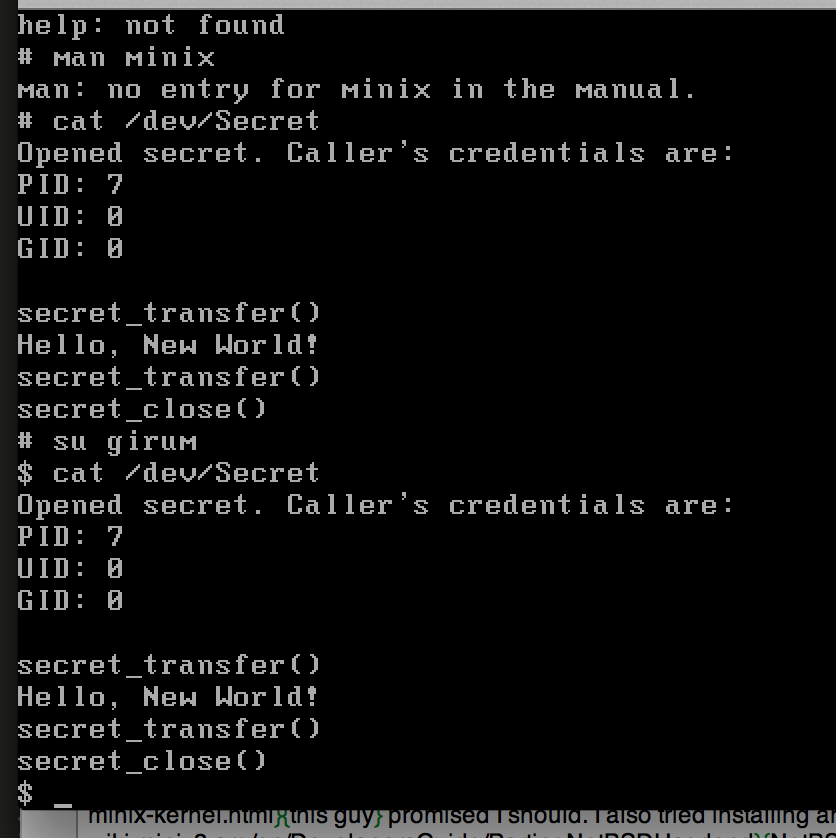
\includegraphics{figure1.png}



\section{Results}
% A section listing problems encountered, solutions attempted, results obtained, and lessons learned as previous labs.
\subsection{Problems encountered}
\begin{itemize}
\item I couldn't compile Minix locally. Eclipse thus wouldn't work for this project. This was because Minix doesn't use standard \texttt{gmake} for its Makefiles. Instead, Minix uses some unknown custom \texttt{make} utility that includes a ton of conditional logic used to auto generate parts of the Makefiles. In the end, I couldn't manage to move Minix's version of \texttt{make} over to my local machine. 
\item Right as I began coding (after 6 hours of reading, config and more reading), my \texttt{getnucred(2)} call refused to work properly. I'm passing it the from \texttt{m\_source} from the \texttt{message *} passed in via the framework, and fill up a \texttt{struct ucred} initialized on the runtime stack. The PID outputs "7" when it should be 697, and both the UID and GID output "0". What's worse, this output is consistent across both of my user accounts.

\end{itemize}

\subsection{Solutions attempted}
\begin{itemize}
\item In attempting to fix the compilation issue (really just a \texttt{make} issue, since Minix doesn't use \texttt{gmake} and instead relies on heavy conditionals to auto generate its Makefiles) I tried copying over the entire \texttt{/usr/src/tools} folder like \href{http://nob.cs.ucdavis.edu/classes/ecs150-2000-01/minix-kernel.html}{this guy} promised I should. I also tried installing and using \href{http://wiki.minix3.org/en/DevelopersGuide/PortingNetBSDUserland}{NetBSD make} to no avail. I gave up and switched to Sublime Text, but I realize now how dependent I am on my IDE. Without Content Assist, I code about as rapidly as a Galapagos Tortoise.
\end{itemize}

\subsection{Results obtained}
Just the modified hello world program so far. And a lot of new knowledge on Minix.

\subsection{Lessions learned}
\begin{itemize}
\item Don't write Makefiles in non-\texttt{gmake}. Not being able to compile Minix on my own machine was by far my biggest headache. But that's more for the writers of Minix to learn from.
\end{itemize}


\section{Other things (as necessary)}
% Other things as necessary: Remember, the meta-goal here is to convince the reader of the report that you successfully implemented a Secret Keeper device, or, failing that, to convey what you did do and that you learned something useful.
Source code that I have submitted via handin to asgn4, and available online at \uline{\href{https://github.com/the-real-girum/cpe453-minix-os}{my GitHub account}}.

\end{document}
